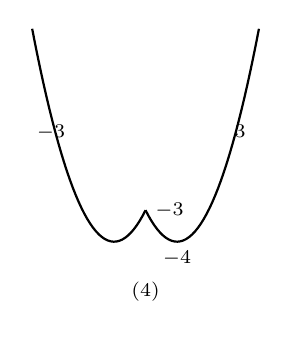
\begin{tikzpicture}[scale=0.4]
\ax{-4.2}{4.2}{-4.8}{3}
\draw[thick,domain=0:3.6,samples=40] plot (\x,{(\x-1)^2-4});
\draw[thick,domain=-3.6:0,samples=40] plot (\x,{(\x+1)^2-4});
\node[below] at (-3,0){\scriptsize $-3$}; \node[below] at (3,0){\scriptsize 3};
\node[right] at (0,-3){\scriptsize $-3$}; \node[below] at (1,-4){\scriptsize $-4$};
\node at (0,-5.6){\scriptsize (4)};
\end{tikzpicture}